% !TEX program = xelatex

\documentclass[hidelinks, 12pt, a4paper]{article}

\usepackage{fontspec}
\setmainfont[Ligatures=TeX]{Linux Libertine O}

\usepackage[hidelinks, colorlinks = true, urlcolor = blue]{hyperref}

\usepackage[utf8]{inputenc}
\usepackage{indentfirst}
\usepackage{graphicx}
\usepackage[left=0.5cm,right=0.5cm,top=2cm,bottom=2cm]{geometry}
\usepackage{lipsum}
\usepackage{caption}
\usepackage{subcaption}
\usepackage{verbatim}
\usepackage{pdfpages}

\usepackage{listings}
\usepackage{xcolor}

\definecolor{codegreen}{rgb}{0,0.6,0}
\definecolor{codegray}{rgb}{0.5,0.5,0.5}
\definecolor{codepurple}{rgb}{0.58,0,0.82}
\definecolor{backcolour}{rgb}{0.95,0.95,0.92}

\lstdefinestyle{mystyle}{
    backgroundcolor=\color{backcolour},   
    commentstyle=\color{codegreen},
    keywordstyle=\color{magenta},
    numberstyle=\tiny\color{codegray},
    stringstyle=\color{codepurple},
    basicstyle=\ttfamily\footnotesize,
    breakatwhitespace=false,         
    breaklines=true,                 
    captionpos=b,                    
    keepspaces=true,                 
    numbers=left,                    
    numbersep=5pt,                  
    showspaces=false,                
    showstringspaces=false,
    showtabs=false,                  
    tabsize=2
}

\lstset{style=mystyle}



\begin{document}
\sloppy % this is legendary

\begin{titlepage}

\begin{figure}[h!]
  \begin{center}
    
\includegraphics[width=3cm]{assets/auth.pdf}
    \label{fig:cover_auth_logo}
  \end{center}
\end{figure}

\centering
\Large Αριστοτέλειο Πανεπιστήμιο Θεσσαλονίκης\\
\Large Πολυτεχνική Σχολή\\
%\large Τμήμα Ηλεκτρολόγων Μηχανικών και Μηχανικών Υπολογιστών\\
%\large Τομέας Τηλεπικοινωνιών

\vspace{\fill}

%\LARGE \textbf{Java socket programming} \\
\LARGE \textbf{Δίκτυα Υπολογιστών Ι}

\vspace{\fill}

\Large Θεόδωρος Κατζάλης \\
\Large ΑΕΜ:9282 \\ 
\Large katzalis@auth.gr

\vspace{\fill}
\raggedright

\centering
\vspace{\fill}
\today

\end{titlepage}

%\maketitle


\pagebreak
{
\renewcommand*\contentsname{Περιεχόμενα}
\hypersetup{linkcolor=black}
\tableofcontents
}
\pagebreak

\section{Δομή του προγράμματος}

\vspace{1cm}

\begin{verbatim}
src
├── ARQ.java
├── Echo.java
├── GPS.java
├── Image.java
├── plot.ipynb
└── UserApplication.java
\end{verbatim}

\section{UserApplication.java}

\lstinputlisting[language=Java]{../src/UserApplication.java}

\pagebreak

\section{Echo.java}

\lstinputlisting[language=Java]{../src/Echo.java}

\section{Image.java}

\lstinputlisting[language=Java]{../src/Image.java}

\section{GPS.java}

\lstinputlisting[language=Java]{../src/GPS.java}

\section{ARQ.java}

\lstinputlisting[language=Java]{../src/ARQ.java}

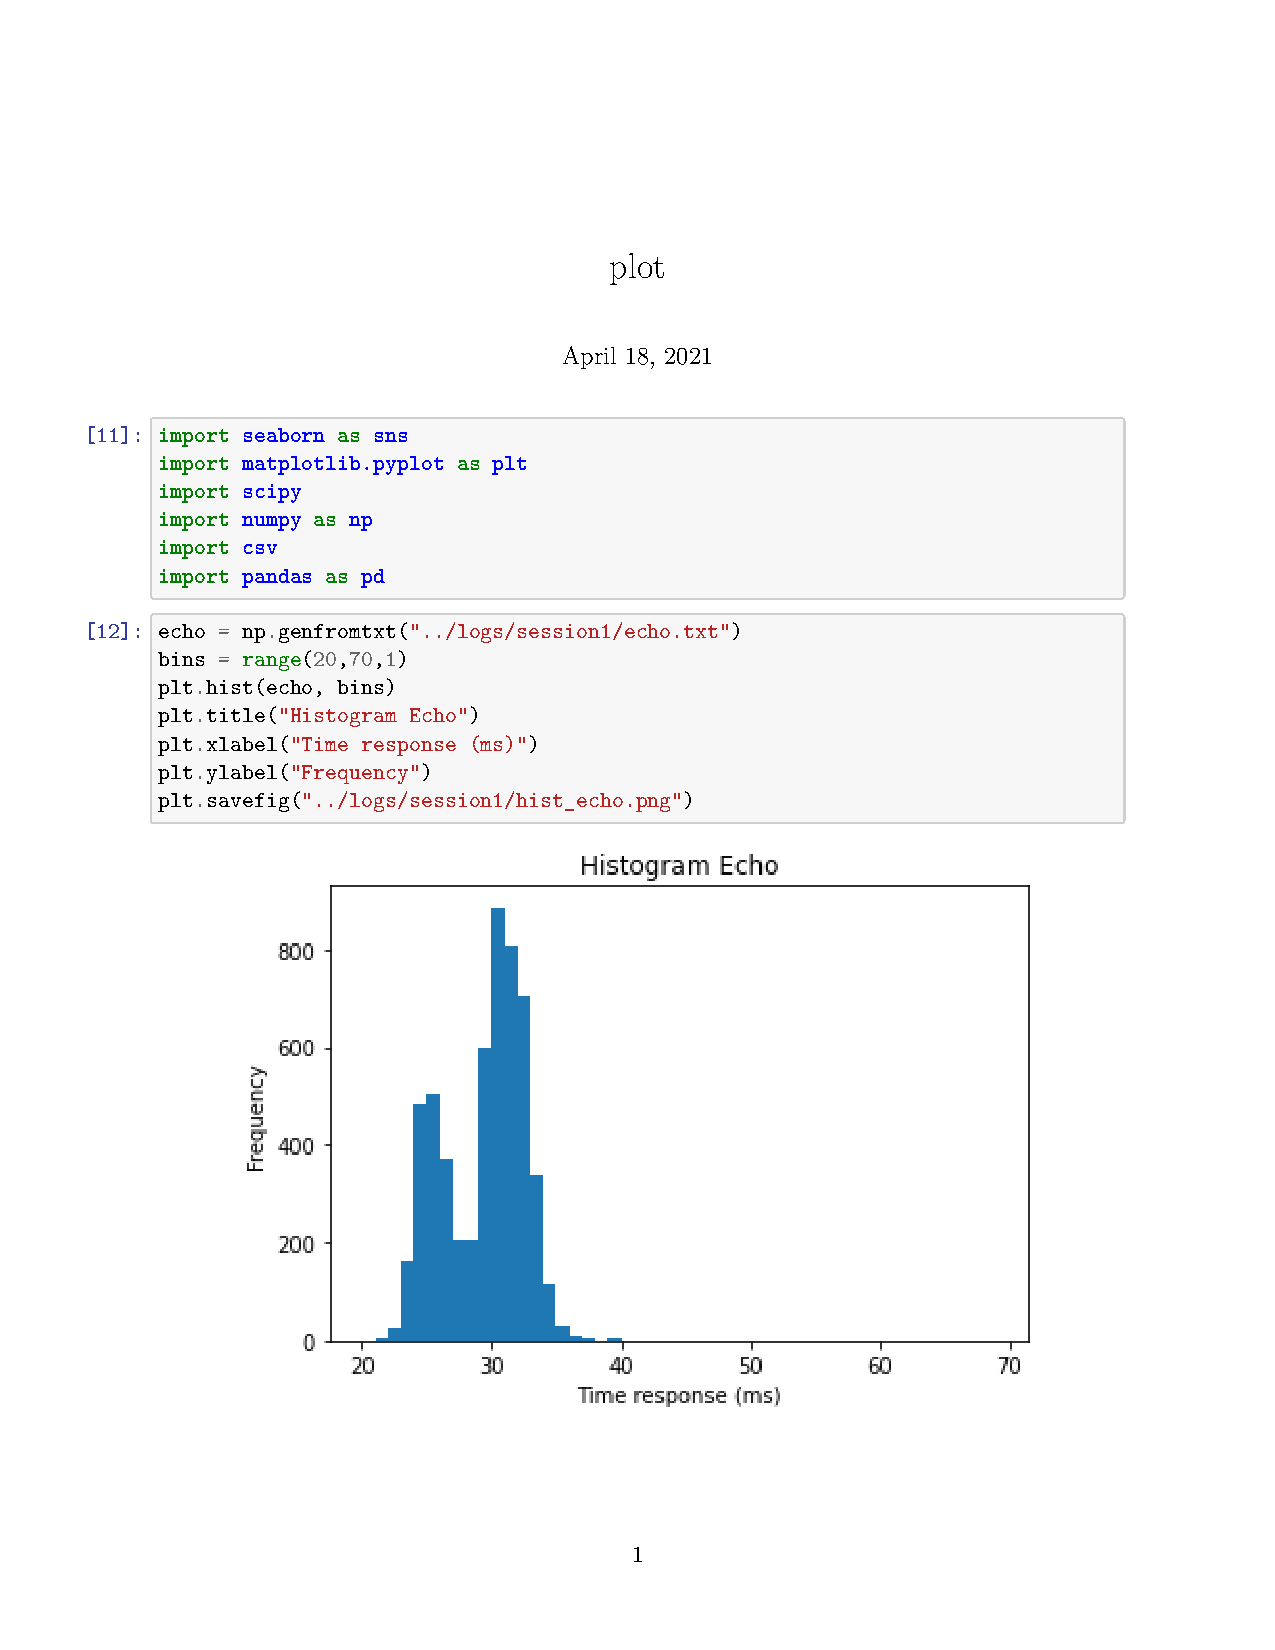
\includepdf[pages=1,pagecommand=\section{Plots}]{./plot.pdf}
\includepdf[pages=2-,pagecommand={}]{./plot.pdf}

\end{document}
